\documentclass{article}
\usepackage{amsmath} % need to be on top for eps files
\usepackage{caption}
\usepackage{subcaption}
\usepackage{graphicx}
\graphicspath{{latex/Images/}}
\usepackage{epstopdf}

%\usepackage[official]{eurosym}
%\usepackage{libertine}
\usepackage{textcomp}
\usepackage{eurosym}

\newcommand{\meuro}{\text{\euro}}
\makeatletter
% Definition taken from eurosym.sty, provides \EUR equivalent for math mode
\newcommand\MEUR[1]{\if@EURleft\text{\euro}\,\fi#1\if@EURleft\else\,\text{\euro}\fi}
\makeatother

%%%%%%%%%Custom
% Allow linking in document.
\usepackage{hyperref}

% Allow including autogenerated LaTex tables from Python.
\usepackage{booktabs}
\usepackage{longtable}
\usepackage{lipsum}

% Determine whether it is local compilation or overleaf compilation
\makeatletter
\begingroup\endlinechar=-1\relax
       \everyeof{\noexpand}%
       \edef\x{\endgroup\def\noexpand\homepath{%
         \@@input|"kpsewhich --var-value=HOME" }}\x
\makeatother
\def\overleafhome{/tmp}% change as appropriate

\ifx\homepath\overleafhome
    % Overleaf compilation.
    \newcommand\blockchaindev{76}
\newcommand\frontenddev{41}
\newcommand\humanresources{36}
\newcommand\bountysubsidising{100000}
\newcommand\buffer{100000}
\newcommand\dailyoperationalcosts{200}
\newcommand\daystooperationalbreakeven{270}
 %\newpage
\else
    % Local compilation
    \newcommand\blockchaindev{76}
\newcommand\frontenddev{41}
\newcommand\humanresources{36}
\newcommand\bountysubsidising{100000}
\newcommand\buffer{100000}
\newcommand\dailyoperationalcosts{200}
\newcommand\daystooperationalbreakeven{270}
 %\newpage
\fi

% Specify compilation name.
\def\filename{main}

% Specify what types of appendices are included in file.
%\def\appendixtypes{no_code}
%\def\appendixtypes{project_code_only}
%\def\appendixtypes{export_code}
\def\appendixtypes{project_and_export_code}



% Use H option in figure placement:
\usepackage{float}

% Use math letters
\usepackage{amsmath} % need to be on top for eps files
\usepackage{mathtools}

% Used for image geometry (already included)
%\usepackage{graphicx}

% Support auto referencing
\usepackage{cleveref}

\crefname{lstlisting}{listing}{listings}
\Crefname{lstlisting}{Listing}{Listings}

% Specify bibliography style:
\usepackage{url}

%%%%%%%%%End Custom


%%%%%%%%%%%%%%%%%%%%%%%%%%%%%%%%%%%%%%%%%%%%%%%%%% Create listings (Matlab)
% % Create a matlab listing
\usepackage{listings}
\usepackage{color} %red, green, blue, yellow, cyan, magenta, black, white
\definecolor{mygreen}{RGB}{28,172,0} % color values Red, Green, Blue
\definecolor{mylilas}{RGB}{170,55,241}

\usepackage[utf8]{inputenc}
\usepackage{geometry}
 \geometry{
 a4paper,
 total={175mm,265mm},
 left=15mm,
 top=15mm,
 }
\usepackage{amsmath}%To be able to use split in equation


%%%% Include eps files:
\usepackage{amsmath} % need to be on top for eps files
\usepackage{graphicx}
%set the relative location for eps files
\graphicspath{ {/Images/} }
\usepackage{listings}
\usepackage{cleveref} %cleverref needs to stand below amsmath package.
\usepackage{graphicx}
\usepackage{float}
%\usepackage{hyperref}
\usepackage{url} %To be able to use url in references
\usepackage{graphicx}
\usepackage{tabularx} % in the preamble
\usepackage{wrapfig}

% To get side by side pictures:{
\usepackage{caption}
\usepackage{subcaption}
\usepackage{graphicx}




%%%%%%%%%%%%%%%%%%%%%%%%%%%%%%%%%%%%%%%%%%%%%%%%%% Create listings (Python)
% set code color pattern (for python)
% Default fixed font does not support bold face
\DeclareFixedFont{\ttb}{T1}{txtt}{bx}{n}{12} % for bold
\DeclareFixedFont{\ttm}{T1}{txtt}{m}{n}{12}  % for normal

% Custom colors
\usepackage{color}
\definecolor{deepblue}{rgb}{0,0,0.5}
\definecolor{deepred}{rgb}{0.6,0,0}
\definecolor{deepgreen}{rgb}{0,0.5,0}

\usepackage{listings}

% Python style for highlighting
\newcommand\pythonstyle{\lstset{
language=Python,
breaklines=true, % wrap lines
postbreak=\mbox{\textcolor{red}{$\hookrightarrow$}\space}, % wrap lines
basicstyle=\ttm,
otherkeywords={self},             % Add keywords here
keywordstyle=\ttb\color{deepblue},
emph={MyClass,__init__},          % Custom highlighting
emphstyle=\ttb\color{deepred},    % Custom highlighting style
stringstyle=\color{deepgreen},
frame=tb,                         % Any extra options here
showstringspaces=false            %
}}

% Python environment
\lstnewenvironment{python}[1][]
{
\pythonstyle
\lstset{#1}
}
{}

% Python for external files
\newcommand\pythonexternal[2][]{{
\pythonstyle
\lstinputlisting[#1]{#2}}}

% Python for inline
\newcommand\pythoninline[1]{{\pythonstyle\lstinline!#1!}}


% Include path to images
\graphicspath{{Images/}{latex/project1/}}

% Include pdf files in report
\usepackage{pdfpages}


\usepackage{cleveref} %cleverref needs to stand below amsmath package.
\usepackage{appendix}
\crefname{appsec}{Appendix}{Appendices} % refer to appendix as appendix iso as section (use with text in
%\title{}
%\subtitle{}
\title{Roadmap: TruCol\\\large A decentralised collaboration protocol for test-driven development}
%\author{Authors:\\a-t-0}



%\def\parent_subpath{/latex/project}% change as appropriate (depending on what Overleaf does)
\usepackage{xstring}


%\def\project_one{/project1}% change as appropriate
%enable multirple columns
\usepackage{multicol}
\usepackage{multirow}

\usepackage{currfile}
\usepackage{currfile-abspath}

% use sidewaysfigure
\usepackage{rotating}

\date{\today}
\begin{document}
\crefname{lstlisting}{listing}{listings}
\Crefname{lstlisting}{Listing}{Listings}
%%%%%%%%%%Configure matlab listing%%%%%%%%%%%%%%%%%%
% Specify matlab listing style
\lstset{language=Matlab,%
    %basicstyle=\color{red},
    breaklines=true,%
    morekeywords={matlab2tikz},
    keywordstyle=\color{blue},%
    morekeywords=[2]{1}, keywordstyle=[2]{\color{black}},
    identifierstyle=\color{black},%
    stringstyle=\color{mylilas},
    commentstyle=\color{mygreen},%
    showstringspaces=false,%without this there will be a symbol in the places where there is a space
    numbers=left,%
    numberstyle={\tiny \color{black}},% size of the numbers
    numbersep=9pt, % this defines how far the numbers are from the text
    emph=[1]{for,end,break},emphstyle=[1]\color{red}, %some words to emphasise
    %emph=[2]{word1,word2}, emphstyle=[2]{style},
}


\maketitle
%\setcounter{chapter}{-1}

% Create abstract.
\ifx\homepath\overleafhome
    % Overleaf compilation.
    \section{Introduction}\label{sec:intro}
Welcome, this document presents our market analysis for the TruCol consultancy. The objective of this document is to provide some basic insight into the order of magnitude of the potential of the TruCol consultancy to generate returns for its potential investors. Based on various pitch templates, \cite{kamps2020}, and private communications, we intend to convey this information through sharing our model and estimate of the following market parameters for the TruCol consultancy:

\begin{itemize}
	\item \textbf{Total addressable market (TAM)}, or total available market, is the total market demand for a product or service, calculated in annual revenue or unit sales if 100\% of the available market is achieved\cite{tam_sam_som}.
	\item \textbf{Serviceable available market (SAM)} is the portion of TAM targeted and served by a company's products or services\cite{tam_sam_som}.
	\item \textbf{Serviceable obtainable market (SOM)}, or share of market, is the percentage of SAM which is realistically reached\cite{tam_sam_som}.
\end{itemize}


\noindent Since we currently have little experience on this topic within our team, we are making our data and assumptions as transparent as possible, both in this document as in our code. This way we hope to improve our model based on your feedback by enabling you to experiment with it yourself. Additionally, because the market analysis consists of a rough estimate, three different estimation methods are used for generating the TAM, SAM and SOM estimates. The redundancy is introduced to establish some frame of reference within the results. % TODO: Improve formulation, referrence frame within the results seems counterintuitive.

The assumptions and data points for the respective models are specified in \cref{sec:assumptions}. Next, the models are described in \cref{sec:model_description} (the Python models themselves are included as appendices in \cref{app:0} to \cref{app:2} respectively). The results of these models are presented in \cref{sec:results}. To shed some light on how sensitive the model is to for example changes in assumptions, a sensitivity analysis is presented for each model in \cref{sec:sensitivity_analysis}. Next the results and sensitivity of the models are discussed in \cref{sec:discussion} and a conclusion is provided in \cref{sec:conclusion}.

We invite you to tinker with the assumptions and models yourself! The data and plots in this report are automatically updated if you run \verb+python -m code.project1.src+. If you experience any difficulties in running the code, simply reach out to us, (click on issues on the github page) and we are happy to get you running the code.
 %\newpage
    \section{Assumptions}\label{sec:assumptions}
\subsection{Top Down}\label{subsec:assumptions_top_down}

\subsection{Bottom Up}\label{subsec:assumptions_bottom_up}
\subsection{Value Theory}\label{subsec:assumptions_value_theory}
To illustrate how the python code exports the figures directly into the report, this second "hw2" is included. Below are the pictures that are created by the code listed in \cref{app:1} and \cref{app:2}.
\begin{figure}[H]
    \centering
    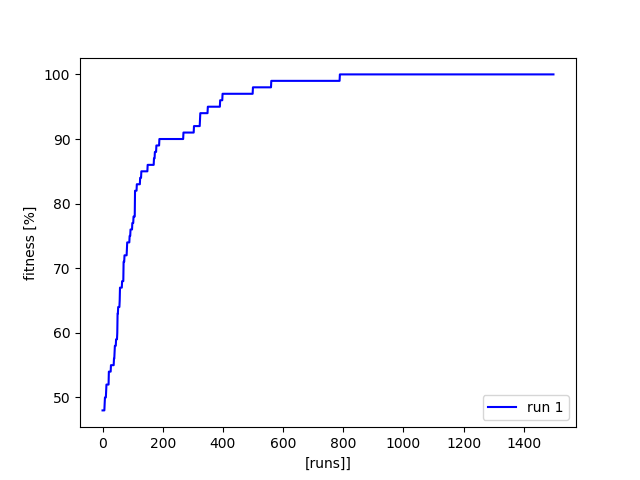
\includegraphics[width=1\textwidth]{Images/4a.png}
    \caption{Performance of some genetic algorithm}
\end{figure}

\begin{figure}[H]
    \centering
    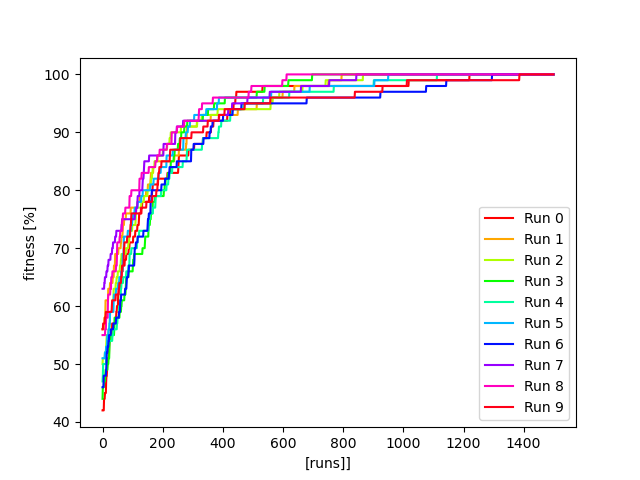
\includegraphics[width=1\textwidth]{Images/4b.png}
    \caption{Performance of some genetic algorithm}
\end{figure} %\newpage
    \section{Model Description}\label{sec:model_descriptions}
\subsection{Top Down}\label{subsec:model_descriptions_top_down}
\subsection{Bottom Up}\label{subsec:model_descriptions_bottom_up}
\subsection{Value Theory}\label{subsec:model_descriptions_value_theory} %\newpage
    
\section{Market Sizing}\label{sec:markets}
% What to convey (Source: Pitch Perfect):
% What is our Market?
% What is the Market Size?
% What is the Market Trajectory

The market sizing parameters are listed in \cref{tab:market_size_params}. The description is given in \cref{subsec:market_introduction}. Ps. \textbf{bold} numbers are model parameters (and possibly assumed), \textcolor{blue}{blue} numbers follow from the model parameters. % TODO: distinguish between data and assumptions in number colour.

\ifx\homepath\overleafhome
    % Overleaf compilation.
    \begin{longtable}{@{}cp{.7\textwidth}@{}}
    \caption{Cost Model Parameters in \euro (/hr or absolute, unlessspecified otherwise)}\label{tab:market_size_params}\\
    \toprule
    {\bfseries Parameter} & {\bfseries Value} \\ \midrule
    \endfirsthead
    \caption{Cost Model Parameters in \euro (/hr or absolute, unlessspecified otherwise) (continued)}\\
    \toprule
    \multicolumn{2}{l}{\scriptsize\emph{\ldots{} continued}}\\
    {\bfseries Parameter} & {\bfseries Value} \\ \midrule
    \endhead
    \multicolumn{2}{r}{\scriptsize\emph{to be continued\ldots}}\\
    \bottomrule
    \endfoot
    \bottomrule
    \endlastfoot
    nr simulations & 300.0\\
    profit dhl billion & 4.099999\\
    profit dhl & 4.100000e+09\\
    profit fedex billion & 1.29\\
    profit fedex & 1.290000e+09\\
    profit ups billion & 7.7\\
    profit ups & 7.700000e+09\\
    profit dhl fedex ups & 1.309000e+10\\
    sam factor & 0.003\\
    tam factor & 0.004\\
    logistics market share dhl fedex ups & 0.15\\
    logistics market share dhl fedex ups percentage & 15.0\\
    avg algo optimisation profit percentage & 0.1\\
    avg algo optimisation profit & 0.001\\
    TruCol cut on profit percentage & 1.0\\
    TruCol cut on profit & 0.01\\
\end{longtable}
 %\newpage
\else
    % Local compilation
    \begin{longtable}{@{}cp{.7\textwidth}@{}}
    \caption{Cost Model Parameters in \euro (/hr or absolute, unlessspecified otherwise)}\label{tab:market_size_params}\\
    \toprule
    {\bfseries Parameter} & {\bfseries Value} \\ \midrule
    \endfirsthead
    \caption{Cost Model Parameters in \euro (/hr or absolute, unlessspecified otherwise) (continued)}\\
    \toprule
    \multicolumn{2}{l}{\scriptsize\emph{\ldots{} continued}}\\
    {\bfseries Parameter} & {\bfseries Value} \\ \midrule
    \endhead
    \multicolumn{2}{r}{\scriptsize\emph{to be continued\ldots}}\\
    \bottomrule
    \endfoot
    \bottomrule
    \endlastfoot
    nr simulations & 300.0\\
    profit dhl billion & 4.099999\\
    profit dhl & 4.100000e+09\\
    profit fedex billion & 1.29\\
    profit fedex & 1.290000e+09\\
    profit ups billion & 7.7\\
    profit ups & 7.700000e+09\\
    profit dhl fedex ups & 1.309000e+10\\
    sam factor & 0.003\\
    tam factor & 0.004\\
    logistics market share dhl fedex ups & 0.15\\
    logistics market share dhl fedex ups percentage & 15.0\\
    avg algo optimisation profit percentage & 0.1\\
    avg algo optimisation profit & 0.001\\
    TruCol cut on profit percentage & 1.0\\
    TruCol cut on profit & 0.01\\
\end{longtable}
 %\newpage
\fi

\subsection{Introduction}\label{subsec:market_introduction}
To use the Top Down Model, \cref{subsec:total_addressable_market} describes the TAM in which the TruCol company will operate. To this end, \cref{subsubsec:tam_logistics} discusses the market size of the logistics market, and the profit within that market. Due to time-constraints and lack of data, some datapoints and assumptions of the logistics market are applied to other sectors such as the automated trading market and pharmaceutics market in \cref{subsubsec:additional_markets} to get some insight in their respective market sizes. Furthermore, \cref{subsubsec:emerging_markets} provides some qualitative insight in the potential future markets that are highly suited for the TruCol protocol. These emerging markets are accordingly expected to be relevant markets to address in the near future.

\subsection{Total Addressable Market}\label{subsec:total_addressable_market}
To compute the TAM, SAM and SOM, some form of market definition can be used. To this end, it is considered valuable to specify what the TruCol company does, where it adds value and how it does that. Furthermore, since these three aforementioned estimates pertain to a potential future, the potential, yet deemed feasible, activities of the TruCol company are included.
\\
The TruCol company provides advice and support to companies on how they can get the most out of the TruCol protocol. To understand this, the following assumptions are shared. Under these assumptions, one can conclude that an economically rational company would try to off-load as much of their required tasks into the TruCol protocol. This is because it would minimise their operational costs and/or improve algorithmic efficiency of their solutions.

\begin{itemize}
	\item \textbf{asu-0:} Solutions to tasks that are completed using the TruCol protocol are deterministically verifiable.
	\item \textbf{asu-1:} Solutions to tasks that are completed using the TruCol protocol are of sufficient quality.
	\item \textbf{asu-2:} Tasks that are completed using the TruCol protocol can be solved for the lowest cost price that is currently available in this world.
	\item \textbf{asu-3:} No personnel needs to be attracted, screened, hired nor fired for tasks that are completed using the TruCol protocol.
	\item \textbf{asu-4:} Companies can benefit from public particular solutions to their task specifications.
	\item \textbf{asu-5:} By sampling from a bigger talent pool (this world), the average performance of the solutions will be better than what is produced by the in-house talent pool, or, for equal solution performance, a faster rate of development can be obtained on average for an equal or lower price.
\end{itemize}



We help companies identify the tasks for which they can use the TruCol protocol, and we assist them in writing safe test specifications that are not easily hackable. This implies that under the given set of assumptions, the TAM for the TruCol protocol can be defined as the total costs that the companies (and consumers) in this world are willing to pay for assistance on using the TruCol protocol.

\subsubsection{TruCol Total Addressable Logistics Market}\label{subsubsec:tam_logistics}

This sub-sub section illustrates a rough method of estimating the logistics sub-segment of the TAM for the TruCol protocol. To do this, an example of algorithmic optimalisation within the logistics market as presented by McKinsey \& Company is generalised conservatively to a rough estimate of the total logistics market size.

A clear example of a logistics company successfully hiring a support for algorithmic optimalisation is documented by McKinsey \& Company in the "how they help their clients" segment of their website\cite{mckinsey_algo}. The study how reports McKinsey's team, among which McKinsey's Strategic Network Analytic Center, helped an Asian logistics company. With McKinseys team, the logistics company realised an \textit{in line haul network cost} reduction of 3.6\% while reducing their \textit{transit time} with 0.8\%, yielding an overall 16\% increase in profit for the logistics company, without compromising the quality. To use this report as a valuable resource to generate some rough estimates on market size, the following assumptions are made:

 \begin{itemize}
 	\item \textbf{asu-6:} The logistics company made a net profit by hiring McKinsey \& Company in this particular ordeal.
	\item \textbf{asu-7:} The example of a 16\% increase in profit is generalizable to a conservative potential \textbf{\avgalgooptimisationprofitpercentage}\% of profit increases through algorithmic optimalisation across the entire logistics industry.
	\item \textbf{asu-8:} Companies are willing to pay at least 1 \% of their potential profit increases for the assistance the TruCol company provides in identifying opportunities for optimisation and for improving test-specification security.
\end{itemize}

\noindent Based on those assumptions, one could find a potential yearly profit increase across the entire logistics sector by summing the net profit of the logistics sector. \cite{cips} claims that this company \cite{transparency_market_research} valued the logistics market at 8.1 trillion in 2016. Additionally, \cite{cips} claims \cite{transparency_market_research} estimates the logistics market value will grow to 15.5 trillion in 2023. However, no figures on profit are found. Therefore, individual companies are explored.

For DHL one can find on pdf page 37/170 in \cite{dhl_2019_annual_report} that the annual profit for DHL in 2019 was \textbf{profitdhlbillion} billion.

For UPS one can find on pdf page 4/257 in \cite{ups_2020_annual_report} that the annual unadjusted operating profit for UPS in 2020 was \textbf{\profitupsbillion} billion. Note, \cite{ups_q21_earnings_call} says UPS had a net operating profit of 1.1 billion in Q1 of 2020, implying they had to almost double their average profit in the remaining three quarters of 2020 to be consistent with an annual \textbf{\profitupsbillion} billion.

For FedEx the net income as reported for 2020 has been \$\textbf{\profitfedexbillion} billion in pdf page 2/17 \cite{fedex_2020_annual_report}.

\begin{itemize}
\item \textbf{Asu-9:} The net income as reported (GAAP) by FedEx can be interpreted as the profit by FedEx.
\end{itemize}

Next, the claim that fragmentation of the global market implied in 2016 that Deutsche Post DHL, Ceva Logistics, UPS, and FedEx, control less than \textbf{\logisticsmarketsharedhlfedexupspercentage}\% of that global market, allows estimating a limit on the net global profit made in the logistics market based on the following assumptions:

\begin{itemize}
	\item \textbf{Asu-10:} The market segment in the global logistics market maintained by the combination of DHL, UPS and FedEx is at most \textbf{\logisticsmarketsharedhlfedexupspercentage}\% in 2020.
	\item \textbf{Asu-11:} The profit in the remaining \textcolor{blue}{85}\% of the global logistics market has the same average yearly profitability per percent market share as the combination of DHL, UPS and FedEx.
\end{itemize}


\section{Results}
\subsection{TAM}
Based on assumptions 1-11 one could estimate an upperbound of
\begin{equation}
	\begin{split}
		net-profit_{DHL+UPS+FedEx}=\textbf{\profitdhlbillion}+\textbf{\profitupsbillion}+\textbf{\profitfedexbillion}=\textcolor{blue}{13.09} billion\\
		\frac{net-profit_{global\_logistics}}{net-profit_{DHL+UPS+FedEx}}=\frac{\textcolor{blue}{0.85}}{\textbf{0.15}}\\
		net-profit_{global\_logistics}=net-profit_{DHL+UPS+FedEx}\frac{\textcolor{blue}{0.85}}{\textbf{0.15}}\\
		net-profit_{global\_logistics}=\frac{\textcolor{blue}{13.09}\cdot\textcolor{blue}{0.85}}{\textbf{0.15}}\\
		net-profit_{global\_logistics}=\textcolor{blue}{74.2} billion
	\end{split}
\end{equation}
\textbf{TODO}: verify in model and text this is TAM or TSAM. TSAM if factor of what is practically addressable is taken into account, e.g. 0.0001\% of market in first year, that is 1 in every 10000 logistics companies. There are \textbf{X} logistics companies, so that requires us to reach out to \textbf{Y} companies and work with \textbf{Z} companies. A follow rate of \textbf{R} is required on a reachout of \textbf{Y}. 

Note, if TSAM is too small, realise the factor 160 might be too small (16\% demonstratable profit gain through algorithmic optimsation, 0.1\% assumed). See Monte-Carlo simulation for a larger spread on assumptions.



\subsection{TruCol Revenue}
Hence, if each of those companies in the logistics sector could increase their profits on average annually by \textbf{\avgalgooptimisationprofitpercentage}\% using algorithmic optimisation, and if they would use the TruCol protocol to do that, and if they would be willing to invest \textbf{\TruColcutonprofitpercentage}\% of that profit in our support and assistance in getting the most out of the TruCol protocol, we would currently estimate that this would yield roughly an income of $\textcolor{blue}{74.2}\cdot \textbf{\avgalgooptimisationprofit}\cdot \textbf{\TruColcutonprofit}=\$\textcolor{blue}{0.74} million$

\subsection{Additional addressable markets}\label{subsubsec:additional_markets}
Since the TruCol company is market agnostic, we also seek to assist in algorithmic optimisation outside the logistics market. Several markets are worth mentioning in particular as we expect them to either heavily rely on algorithmic optimisations, or because they are particularly suited for the TruCol protocol.
\begin{itemize}
	\item \textbf{(Automated) trading} In the highly competitive market of (automated) trading, algorithmic optimisations are key to making successful trades.
	\item \textbf{Space Sector} The space engineering sector already has a relatively high test driven development\cite{todo}, this lowers the adoption costs of the TruCol protocol relative to most industries. Furthermore, space applications are heavily mass constrained, which generally makes them highly energy constrained as well. These energy constraints emphasise the importance of algorithmic optimisations, for example in telecommunications satellites and swarm robots.
	\item \textbf{Innovative Materials Research} The domain of material science has been adopting algorithmic search strategies to find new materials  \cite{allahyari2020coevolutionary}.
	\item \textbf{Pharmaceutical Industry} Another example of a large market that has been shifting to adopt algorithmic search strategies to find new medicines.
\end{itemize}
Each of these are multi-billion dollar markets which can contribute to the TAM of the TruCol company.
% NP problems
% Neuromorphic
% Space
% Logistics
% Chemical compound development
% Protein folding
\subsubsection{Emerging markets}\label{subsubsec:emerging_markets}
Beyond those listed markets, the following emerging markets could be great opportunities for the TruCol company to latch in and grow along in.
\begin{itemize}
	\item \textbf{Neuromorphic Computing} This field is developing new complexity theory to adapt to the unconventional computation methods. This is an interesting opportunity to explore the versatility of the TruCol protocol.
	\item \textbf{Quantum Computing} This is another upcoming field with many new algorithmic implementations. The newness of the field may suggest that the amount of optimisation and exploration to be done is relatively high, possibly indicating a relatively large potential for the TruCol protocol. However, currently our team does not yet contain experience in this type of algorithmic developments.
	\item \textbf{Artificial Intelligence} With the introduction of GPT-3 and GitHub Copilot, the world has seen examples of AI engines that are able to generate code for some basic tasks. The TruCol protocol could catalyse the usage of such AI engines that are able to write code based on requirement specification. We expect that users of the TruCol protocol will develop a tactical advantage on requirement specifications for AI engines.
\end{itemize}

% AI requirements specicfication
% AI engines

%\subsection{Market Trajectory}\label{subsec:model_description_market_trajectory}
 %\newpage
    \section{Results}\label{sec:results}
\subsection{Top Down Model}\label{subsec:results_top_down}
%\subsection{Bottom Up Model}\label{subsec:results_bottom_up}
%\subsection{Value Theory Model}\label{subsec:results_value_theory}
The code listed in the appendices generated the following estimates for the total addressable market sizes for the TruCol company.
\begin{figure}[H]
    \centering
    \includegraphics[width=0.5\linewidth]{Images/revenue_per_sector.png}
    \caption{A scatterplot generated by a Monte-Carlo simulation to provide an impression on the estimated projected total addressable market per sector for the TruCol company.}
    \label{fig:per_sector}
\end{figure}

\begin{figure}[H]
    \centering
    \includegraphics[width=0.5\linewidth]{Images/revenue_sum.png}
    \caption{A scatterplot generated by a Monte-Carlo simulation to provide an estimate on the projected total addressable market for the TruCol company.}
    \label{fig:summed}
\end{figure}
 %\newpage
    \section{Sensitivity Analysis}\label{sec:sensitivity_analysis}
\subsection{Top Down}\label{subsec:sensitivity_analysis_top_down}
%\subsection{Bottom Up}\label{subsec:sensitivity_analysis_bottom_up}
%\subsection{Value Theory}\label{subsec:sensitivity_analysis_value_theory}
Omitted due to time constraints. Can be generated upon request. %\newpage
    \section{Discussion}\label{sec:discussion}
We expect that the main points for improvement in this analysis are the datapoints that are used. In particular, the generalisation of the profit margin of the logistics sector to other sectors could be replaced by the actual data of the other sectors. Furthermore, the profit margin of the logistics sector could be searched directly instead of deriving it based on the of its larger companies.
 %\newpage
    \section{Conclusion}\label{sec:conclusion}
A rough estimate based on various datasources has been generated to estimate the yearly revenue of the TruCol company. Additional iterations with improved datapoints is recommended to obtain a more accurate estimate. The market analysis does not yet include the growth that may be captured in diversification, emerging markets such as neuromorphic computing and in-house automation/AI-engines. Before taking these potentials into account, however, a more accurate assessment of the starting market is recommended. %\newpage
\else
    % Local compilation
    \section{Introduction}\label{sec:intro}
Welcome, this document presents our market analysis for the TruCol company. The objective of this document is to provide some basic insight into the order of magnitude of the potential of the TruCol company to generate returns for its potential investors. Based on various pitch templates, \cite{kamps2020}, and private communications, we intend to convey this information through sharing our model and estimate of the following market parameters for the TruCol company:

\begin{itemize}
	\item \textbf{Total addressable market (TAM)}, or total available market, is the total market demand for a product or service, calculated in annual revenue or unit sales if 100\% of the available market is achieved\cite{tam_sam_som}.
	\item \textbf{Serviceable available market (SAM)} is the portion of TAM targeted and served by a company's products or services\cite{tam_sam_som}.
	\item \textbf{Serviceable obtainable market (SOM)}, or share of market, is the percentage of SAM which is realistically reached\cite{tam_sam_som}.
\end{itemize}


\noindent Since we currently have little experience on this topic within our team, we are making our data and assumptions as transparent as possible, both in this document as in our code. This way, we hope to improve our model based on your feedback by enabling you to experiment with it yourself. Additionally, because the market analysis consists of a rough estimate, three different estimation methods are considered for generating the TAM, SAM and SOM estimates. The redundancy is introduced in an attempt to establish some frame of reference within the results. % TODO: Improve formulation, reference frame within the results seems counterintuitive.
The assumptions and data points for the respective models are specified explicitly in this document with an identifier, and where relevant, this identifier is used in the comment of the code to link the document and code.

% TODO: order

The mathematical models are described in \cref{sec:market_analysis_model}.
\ifnum\pdfstrcmp{no_code}{\appendixtypes}=0
The Python models can be inspected at \url{https://github.com/TruCol/Market_analysis/tree/main/src}, or appended upon request.
\fi
\ifnum\pdfstrcmp{project_code_only}{\appendixtypes}=0
(the Python models themselves are included as appendices.
\fi
\ifnum\pdfstrcmp{export_code}{\appendixtypes}=0
The Python models can be inspected at \url{https://github.com/TruCol/Market_analysis/tree/main/src}, or appended upon request.
\fi
\ifnum\pdfstrcmp{project_and_export_code}{\appendixtypes}=0
(the Python models themselves are included as appendices.
\fi



The results of these models are presented in \cref{sec:results}. To shed some light on how sensitive the model is to for example changes in assumptions, a sensitivity analysis is presented for each model in \cref{sec:sensitivity_analysis}. Next, the results and sensitivity of the models are discussed in \cref{sec:discussion} and a conclusion is provided in \cref{sec:conclusion}.

We invite you to tinker with the assumptions and models yourself! The data and plots in this report are automatically updated if you run \verb+python -m code.project1.src+. If you experience any difficulties in running the code, simply reach out to us, (click on issues on the GitHub page) and we are happy to get you running the code.
 %\newpage
    \section{TruCol Company Business Model}\label{sec:trucol_company_business_model}
Since the market size estimation models are somewhat of an abstract/subjective task, three different approaches are used in an attempt to establish some reference material with respect to accuracy.


Before the model is presented, it is important to realise that we propose an optimisation service. This means that if a certain activity, e.g. a logistics company has operational cost of 5 \$million/day, our service is only able to earn at most the margin of improvement we are able to bring our customer. Suppose the independent usage of the TruCol provides the customer with a 2\% optimisation in their operational costs, yielding them $5.000.000\cdot 0.02=100.000/day$\$. Suppose our expertise is able to enable them to yield a 3\% optimisation by identifying the relevant development/system processes and supporting them in improved test specification. In that assumption our company would bring them an additional 3-2=1\% which would translate roughly to $50.000$\$. That would be the value we bring to the logistics company in this hypothetical scenario.

In reality this example is oversimplified, the 2\% the company could get by themselves would involve some risk pertaining to inaccurate test specification which could lead to loss of the bounty. Our company reduces this risk by providing test-specification security expertise. Furthermore, our interaction with the client may bring the client experience that can be applied in future applications of the TruCol protocol, hence the value to we bring to the client is larger than the amount they gain in terms of optimisation w.r.t. the case where they use the protocol themselves.
 %\newpage
    \section{Market Analysis Models}\label{sec:market_analysis_model}
This section describes the model that is used to perform the market analysis for the TruCol company service. The model will be used to estimate the yearly revenue that is projected for this company. Typical estimation models to do this for startups are:
\begin{itemize}
	\item \textit{Top Down Model} - Starts with a large population with known size that make up the target market, and then narrows the market size down to the specific market segment.
	\item \textit{Bottom Up Model} - Takes current pricing and/or usage of product as a starting point and extrapolates up/outwards to compute the potential market size.
	\item \textit{Value Theory Model} - estimates the value provided to customers and estimates how much of that value can be reflected in the product pricing.
\end{itemize}

\noindent Since the TruCol company does not yet have a large body of current pricing and product usage, the Bottom Up Model is not used in this market analysis document. Similarly, the Value Theory Model is omitted in this market analysis as it is most powerful on historical data which is not yet available for the TruCol protocol. Since the market sizes of most sectors in which the TruCol company intends to operate, the Top Down Model is used to derive a rough estimate of the projected yearly revenue for the TruCol company.
 %\newpage
    
\section{Market Sizing}\label{sec:markets}
% What to convey (Source: Pitch Perfect):
% What is our Market?
% What is the Market Size?
% What is the Market Trajectory

The market sizing parameters are listed in \cref{tab:market_size_params}. The description is given in \cref{subsec:market_introduction}. Ps. \textbf{bold} numbers are model parameters (and possibly assumed), \textcolor{blue}{blue} numbers follow from the model parameters. % TODO: distinguish between data and assumptions in number colour.

\ifx\homepath\overleafhome
    % Overleaf compilation.
    \begin{longtable}{@{}cp{.7\textwidth}@{}}
    \caption{Cost Model Parameters in \euro (/hr or absolute, unlessspecified otherwise)}\label{tab:market_size_params}\\
    \toprule
    {\bfseries Parameter} & {\bfseries Value} \\ \midrule
    \endfirsthead
    \caption{Cost Model Parameters in \euro (/hr or absolute, unlessspecified otherwise) (continued)}\\
    \toprule
    \multicolumn{2}{l}{\scriptsize\emph{\ldots{} continued}}\\
    {\bfseries Parameter} & {\bfseries Value} \\ \midrule
    \endhead
    \multicolumn{2}{r}{\scriptsize\emph{to be continued\ldots}}\\
    \bottomrule
    \endfoot
    \bottomrule
    \endlastfoot
    nr simulations & 300.0\\
    profit dhl billion & 4.099999\\
    profit dhl & 4.100000e+09\\
    profit fedex billion & 1.29\\
    profit fedex & 1.290000e+09\\
    profit ups billion & 7.7\\
    profit ups & 7.700000e+09\\
    profit dhl fedex ups & 1.309000e+10\\
    sam factor & 0.003\\
    tam factor & 0.004\\
    logistics market share dhl fedex ups & 0.15\\
    logistics market share dhl fedex ups percentage & 15.0\\
    avg algo optimisation profit percentage & 0.1\\
    avg algo optimisation profit & 0.001\\
    TruCol cut on profit percentage & 1.0\\
    TruCol cut on profit & 0.01\\
\end{longtable}
 %\newpage
\else
    % Local compilation
    \begin{longtable}{@{}cp{.7\textwidth}@{}}
    \caption{Cost Model Parameters in \euro (/hr or absolute, unlessspecified otherwise)}\label{tab:market_size_params}\\
    \toprule
    {\bfseries Parameter} & {\bfseries Value} \\ \midrule
    \endfirsthead
    \caption{Cost Model Parameters in \euro (/hr or absolute, unlessspecified otherwise) (continued)}\\
    \toprule
    \multicolumn{2}{l}{\scriptsize\emph{\ldots{} continued}}\\
    {\bfseries Parameter} & {\bfseries Value} \\ \midrule
    \endhead
    \multicolumn{2}{r}{\scriptsize\emph{to be continued\ldots}}\\
    \bottomrule
    \endfoot
    \bottomrule
    \endlastfoot
    nr simulations & 300.0\\
    profit dhl billion & 4.099999\\
    profit dhl & 4.100000e+09\\
    profit fedex billion & 1.29\\
    profit fedex & 1.290000e+09\\
    profit ups billion & 7.7\\
    profit ups & 7.700000e+09\\
    profit dhl fedex ups & 1.309000e+10\\
    sam factor & 0.003\\
    tam factor & 0.004\\
    logistics market share dhl fedex ups & 0.15\\
    logistics market share dhl fedex ups percentage & 15.0\\
    avg algo optimisation profit percentage & 0.1\\
    avg algo optimisation profit & 0.001\\
    TruCol cut on profit percentage & 1.0\\
    TruCol cut on profit & 0.01\\
\end{longtable}
 %\newpage
\fi

\subsection{Introduction}\label{subsec:market_introduction}
To use the Top Down Model, \cref{subsec:total_addressable_market} describes the TAM in which the TruCol company will operate. To this end, \cref{subsubsec:tam_logistics} discusses the market size of the logistics market, and the profit within that market. Due to time-constraints and lack of data, some datapoints and assumptions of the logistics market are applied to other sectors such as the automated trading market and pharmaceutics market in \cref{subsubsec:additional_markets} to get some insight in their respective market sizes. Furthermore, \cref{subsubsec:emerging_markets} provides some qualitative insight in the potential future markets that are highly suited for the TruCol protocol. These emerging markets are accordingly expected to be relevant markets to address in the near future.

\subsection{Total Addressable Market}\label{subsec:total_addressable_market}
To compute the TAM, SAM and SOM, some form of market definition can be used. To this end, it is considered valuable to specify what the TruCol company does, where it adds value and how it does that. Furthermore, since these three aforementioned estimates pertain to a potential future, the potential, yet deemed feasible, activities of the TruCol company are included.
\\
The TruCol company provides advice and support to companies on how they can get the most out of the TruCol protocol. To understand this, the following assumptions are shared. Under these assumptions, one can conclude that an economically rational company would try to off-load as much of their required tasks into the TruCol protocol. This is because it would minimise their operational costs and/or improve algorithmic efficiency of their solutions.

\begin{itemize}
	\item \textbf{asu-0:} Solutions to tasks that are completed using the TruCol protocol are deterministically verifiable.
	\item \textbf{asu-1:} Solutions to tasks that are completed using the TruCol protocol are of sufficient quality.
	\item \textbf{asu-2:} Tasks that are completed using the TruCol protocol can be solved for the lowest cost price that is currently available in this world.
	\item \textbf{asu-3:} No personnel needs to be attracted, screened, hired nor fired for tasks that are completed using the TruCol protocol.
	\item \textbf{asu-4:} Companies can benefit from public particular solutions to their task specifications.
	\item \textbf{asu-5:} By sampling from a bigger talent pool (this world), the average performance of the solutions will be better than what is produced by the in-house talent pool, or, for equal solution performance, a faster rate of development can be obtained on average for an equal or lower price.
\end{itemize}



We help companies identify the tasks for which they can use the TruCol protocol, and we assist them in writing safe test specifications that are not easily hackable. This implies that under the given set of assumptions, the TAM for the TruCol protocol can be defined as the total costs that the companies (and consumers) in this world are willing to pay for assistance on using the TruCol protocol.

\subsubsection{TruCol Total Addressable Logistics Market}\label{subsubsec:tam_logistics}

This sub-sub section illustrates a rough method of estimating the logistics sub-segment of the TAM for the TruCol protocol. To do this, an example of algorithmic optimalisation within the logistics market as presented by McKinsey \& Company is generalised conservatively to a rough estimate of the total logistics market size.

A clear example of a logistics company successfully hiring a support for algorithmic optimalisation is documented by McKinsey \& Company in the "how they help their clients" segment of their website\cite{mckinsey_algo}. The study how reports McKinsey's team, among which McKinsey's Strategic Network Analytic Center, helped an Asian logistics company. With McKinseys team, the logistics company realised an \textit{in line haul network cost} reduction of 3.6\% while reducing their \textit{transit time} with 0.8\%, yielding an overall 16\% increase in profit for the logistics company, without compromising the quality. To use this report as a valuable resource to generate some rough estimates on market size, the following assumptions are made:

 \begin{itemize}
 	\item \textbf{asu-6:} The logistics company made a net profit by hiring McKinsey \& Company in this particular ordeal.
	\item \textbf{asu-7:} The example of a 16\% increase in profit is generalizable to a conservative potential \textbf{\avgalgooptimisationprofitpercentage}\% of profit increases through algorithmic optimalisation across the entire logistics industry.
	\item \textbf{asu-8:} Companies are willing to pay at least 1 \% of their potential profit increases for the assistance the TruCol company provides in identifying opportunities for optimisation and for improving test-specification security.
\end{itemize}

\noindent Based on those assumptions, one could find a potential yearly profit increase across the entire logistics sector by summing the net profit of the logistics sector. \cite{cips} claims that this company \cite{transparency_market_research} valued the logistics market at 8.1 trillion in 2016. Additionally, \cite{cips} claims \cite{transparency_market_research} estimates the logistics market value will grow to 15.5 trillion in 2023. However, no figures on profit are found. Therefore, individual companies are explored.

For DHL one can find on pdf page 37/170 in \cite{dhl_2019_annual_report} that the annual profit for DHL in 2019 was \textbf{profitdhlbillion} billion.

For UPS one can find on pdf page 4/257 in \cite{ups_2020_annual_report} that the annual unadjusted operating profit for UPS in 2020 was \textbf{\profitupsbillion} billion. Note, \cite{ups_q21_earnings_call} says UPS had a net operating profit of 1.1 billion in Q1 of 2020, implying they had to almost double their average profit in the remaining three quarters of 2020 to be consistent with an annual \textbf{\profitupsbillion} billion.

For FedEx the net income as reported for 2020 has been \$\textbf{\profitfedexbillion} billion in pdf page 2/17 \cite{fedex_2020_annual_report}.

\begin{itemize}
\item \textbf{Asu-9:} The net income as reported (GAAP) by FedEx can be interpreted as the profit by FedEx.
\end{itemize}

Next, the claim that fragmentation of the global market implied in 2016 that Deutsche Post DHL, Ceva Logistics, UPS, and FedEx, control less than \textbf{\logisticsmarketsharedhlfedexupspercentage}\% of that global market, allows estimating a limit on the net global profit made in the logistics market based on the following assumptions:

\begin{itemize}
	\item \textbf{Asu-10:} The market segment in the global logistics market maintained by the combination of DHL, UPS and FedEx is at most \textbf{\logisticsmarketsharedhlfedexupspercentage}\% in 2020.
	\item \textbf{Asu-11:} The profit in the remaining \textcolor{blue}{85}\% of the global logistics market has the same average yearly profitability per percent market share as the combination of DHL, UPS and FedEx.
\end{itemize}


\section{Results}
\subsection{TAM}
Based on assumptions 1-11 one could estimate an upperbound of
\begin{equation}
	\begin{split}
		net-profit_{DHL+UPS+FedEx}=\textbf{\profitdhlbillion}+\textbf{\profitupsbillion}+\textbf{\profitfedexbillion}=\textcolor{blue}{13.09} billion\\
		\frac{net-profit_{global\_logistics}}{net-profit_{DHL+UPS+FedEx}}=\frac{\textcolor{blue}{0.85}}{\textbf{0.15}}\\
		net-profit_{global\_logistics}=net-profit_{DHL+UPS+FedEx}\frac{\textcolor{blue}{0.85}}{\textbf{0.15}}\\
		net-profit_{global\_logistics}=\frac{\textcolor{blue}{13.09}\cdot\textcolor{blue}{0.85}}{\textbf{0.15}}\\
		net-profit_{global\_logistics}=\textcolor{blue}{74.2} billion
	\end{split}
\end{equation}
\textbf{TODO}: verify in model and text this is TAM or TSAM. TSAM if factor of what is practically addressable is taken into account, e.g. 0.0001\% of market in first year, that is 1 in every 10000 logistics companies. There are \textbf{X} logistics companies, so that requires us to reach out to \textbf{Y} companies and work with \textbf{Z} companies. A follow rate of \textbf{R} is required on a reachout of \textbf{Y}. 

Note, if TSAM is too small, realise the factor 160 might be too small (16\% demonstratable profit gain through algorithmic optimsation, 0.1\% assumed). See Monte-Carlo simulation for a larger spread on assumptions.



\subsection{TruCol Revenue}
Hence, if each of those companies in the logistics sector could increase their profits on average annually by \textbf{\avgalgooptimisationprofitpercentage}\% using algorithmic optimisation, and if they would use the TruCol protocol to do that, and if they would be willing to invest \textbf{\TruColcutonprofitpercentage}\% of that profit in our support and assistance in getting the most out of the TruCol protocol, we would currently estimate that this would yield roughly an income of $\textcolor{blue}{74.2}\cdot \textbf{\avgalgooptimisationprofit}\cdot \textbf{\TruColcutonprofit}=\$\textcolor{blue}{0.74} million$

\subsection{Additional addressable markets}\label{subsubsec:additional_markets}
Since the TruCol company is market agnostic, we also seek to assist in algorithmic optimisation outside the logistics market. Several markets are worth mentioning in particular as we expect them to either heavily rely on algorithmic optimisations, or because they are particularly suited for the TruCol protocol.
\begin{itemize}
	\item \textbf{(Automated) trading} In the highly competitive market of (automated) trading, algorithmic optimisations are key to making successful trades.
	\item \textbf{Space Sector} The space engineering sector already has a relatively high test driven development\cite{todo}, this lowers the adoption costs of the TruCol protocol relative to most industries. Furthermore, space applications are heavily mass constrained, which generally makes them highly energy constrained as well. These energy constraints emphasise the importance of algorithmic optimisations, for example in telecommunications satellites and swarm robots.
	\item \textbf{Innovative Materials Research} The domain of material science has been adopting algorithmic search strategies to find new materials  \cite{allahyari2020coevolutionary}.
	\item \textbf{Pharmaceutical Industry} Another example of a large market that has been shifting to adopt algorithmic search strategies to find new medicines.
\end{itemize}
Each of these are multi-billion dollar markets which can contribute to the TAM of the TruCol company.
% NP problems
% Neuromorphic
% Space
% Logistics
% Chemical compound development
% Protein folding
\subsubsection{Emerging markets}\label{subsubsec:emerging_markets}
Beyond those listed markets, the following emerging markets could be great opportunities for the TruCol company to latch in and grow along in.
\begin{itemize}
	\item \textbf{Neuromorphic Computing} This field is developing new complexity theory to adapt to the unconventional computation methods. This is an interesting opportunity to explore the versatility of the TruCol protocol.
	\item \textbf{Quantum Computing} This is another upcoming field with many new algorithmic implementations. The newness of the field may suggest that the amount of optimisation and exploration to be done is relatively high, possibly indicating a relatively large potential for the TruCol protocol. However, currently our team does not yet contain experience in this type of algorithmic developments.
	\item \textbf{Artificial Intelligence} With the introduction of GPT-3 and GitHub Copilot, the world has seen examples of AI engines that are able to generate code for some basic tasks. The TruCol protocol could catalyse the usage of such AI engines that are able to write code based on requirement specification. We expect that users of the TruCol protocol will develop a tactical advantage on requirement specifications for AI engines.
\end{itemize}

% AI requirements specicfication
% AI engines

%\subsection{Market Trajectory}\label{subsec:model_description_market_trajectory}
 %\newpage
    \section{Results}\label{sec:results}
\subsection{Top Down Model}\label{subsec:results_top_down}
%\subsection{Bottom Up Model}\label{subsec:results_bottom_up}
%\subsection{Value Theory Model}\label{subsec:results_value_theory}
The code listed in the appendices generated the following estimates for the total addressable market sizes for the TruCol company.
\begin{figure}[H]
    \centering
    \ifx\homepath\overleafhome
		\includegraphics[width=0.5\linewidth]{Images/revenue_per_sector.png}
	\else
    \includegraphics[width=0.5\linewidth]{latex/Images/revenue_per_sector.png}
	\fi

    \caption{A scatterplot generated by a Monte-Carlo simulation to provide an impression on the estimated projected total addressable market per sector for the TruCol company.}
    \label{fig:per_sector}
\end{figure}

\begin{figure}[H]
    \centering
    \ifx\homepath\overleafhome
    \includegraphics[width=0.5\linewidth]{Images/revenue_sum.png}
	\else
    \includegraphics[width=0.5\linewidth]{latex/Images/revenue_sum.png}
	\fi

    \caption{A scatterplot generated by a Monte-Carlo simulation to provide an estimate on the projected total addressable market for the TruCol company.}
    \label{fig:summed}
\end{figure}
 %\newpage
    \section{Sensitivity Analysis}\label{sec:sensitivity_analysis}
\subsection{Top Down}\label{subsec:sensitivity_analysis_top_down}
%\subsection{Bottom Up}\label{subsec:sensitivity_analysis_bottom_up}
%\subsection{Value Theory}\label{subsec:sensitivity_analysis_value_theory}
Omitted due to time constraints. Can be generated upon request.
 %\newpage
    \section{Discussion}\label{sec:discussion}
We expect that the main points for improvement in this analysis are the datapoints that are used. In particular, the generalisation of the profit margin of the logistics sector to other sectors could be replaced by the actual data of the other sectors. Furthermore, the profit margin of the logistics sector could be searched directly instead of deriving it based on the of its larger companies.
 %\newpage
    \section{Conclusion}\label{sec:conclusion}
A rough estimate based on various datasources has been generated to estimate the yearly revenue of the TruCol company. Additional iterations with improved datapoints is recommended to obtain a more accurate estimate. The market analysis does not yet include the growth that may be captured in diversification, emerging markets such as neuromorphic computing and in-house automation/AI-engines. Before taking these potentials into account, however, a more accurate assessment of the starting market is recommended.
 %\newpage
\fi

% Include bibliography
\bibliographystyle{plain} %plain style
\bibliography{references_market_analysis}
\addcontentsline{toc}{chapter}{Bibliography}

% Include appendices
\ifnum\pdfstrcmp{no_code}{\appendixtypes}=0
  % Don't include any code appendices. Feel free to add manual appendices here.
  \newpage
  \begin{appendices}
    \ifx\homepath\overleafhome
        % Overleaf compilation.
        %\input{Appendices/manual_appendices.tex} %\newpage
    \else
        % Local compilation
        %\input{latex/Appendices/manual_appendices_from_root.tex} %\newpage
    \fi
  \end{appendices}
\fi

% Include project code only.
\ifnum\pdfstrcmp{project_code_only}{\appendixtypes}=0
  \newpage
  \begin{appendices}
    \ifx\homepath\overleafhome
        % Overleaf compilation.
        \section{Appendix \/src/Activity.py}\label{app:Activity.py}
\pythonexternal{latex/../src/Activity.py}
 \newpage
\section{Appendix \/src/Cost\_model.py}\label{app:Cost_model.py}
\pythonexternal{latex/../src/Cost_model.py}
 \newpage
\section{Appendix \/src/Create\_python\_gantt.py}\label{app:Create_python_gantt.py}
\pythonexternal{latex/../src/Create_python_gantt.py}
 \newpage
\section{Appendix \/src/Gantt.py}\label{app:Gantt.py}
\pythonexternal{latex/../src/Gantt.py}
 \newpage
\section{Appendix \/src/\_\_main\_\_.py}\label{app:__main__.py}
\pythonexternal{latex/../src/__main__.py}
 \newpage
\section{Appendix \/src/arg\_parser.py}\label{app:arg_parser.py}
\pythonexternal{latex/../src/arg_parser.py}
 \newpage
 %\newpage
    \else
        % Local compilation
        \section{Appendix \/src/Activity.py}\label{app:Activity.py}
\pythonexternal{latex/../src/Activity.py}
 \newpage
\section{Appendix \/src/Cost\_model.py}\label{app:Cost_model.py}
\pythonexternal{latex/../src/Cost_model.py}
 \newpage
\section{Appendix \/src/Create\_python\_gantt.py}\label{app:Create_python_gantt.py}
\pythonexternal{latex/../src/Create_python_gantt.py}
 \newpage
\section{Appendix \/src/Gantt.py}\label{app:Gantt.py}
\pythonexternal{latex/../src/Gantt.py}
 \newpage
\section{Appendix \/src/\_\_main\_\_.py}\label{app:__main__.py}
\pythonexternal{latex/../src/__main__.py}
 \newpage
\section{Appendix \/src/arg\_parser.py}\label{app:arg_parser.py}
\pythonexternal{latex/../src/arg_parser.py}
 \newpage
 %\newpage
    \fi
  \end{appendices}
\fi

% Include only the code used to export the images, code etc. Skip project code.
\ifnum\pdfstrcmp{export_code}{\appendixtypes}=0
  \newpage
  \begin{appendices}
    \ifx\homepath\overleafhome
        % Overleaf compilation.
        \section{Appendix \/src/export\_data/Hardcoded\_data.py}\label{app:Hardcoded_data.py}
\pythonexternal{latex/../src/export_data/Hardcoded_data.py}
 \newpage
\section{Appendix \/src/export\_data/Milestone.py}\label{app:Milestone.py}
\pythonexternal{latex/../src/export_data/Milestone.py}
 \newpage
\section{Appendix \/src/export\_data/Plot\_to\_tex.py}\label{app:Plot_to_tex.py}
\pythonexternal{latex/../src/export_data/Plot_to_tex.py}
 \newpage
\section{Appendix \/src/export\_data/create\_dynamic\_diagrams.py}\label{app:create_dynamic_diagrams.py}
\pythonexternal{latex/../src/export_data/create_dynamic_diagrams.py}
 \newpage
\section{Appendix \/src/export\_data/create\_static\_diagrams.py}\label{app:create_static_diagrams.py}
\pythonexternal{latex/../src/export_data/create_static_diagrams.py}
 \newpage
\section{Appendix \/src/export\_data/export\_data.py}\label{app:export_data.py}
\pythonexternal{latex/../src/export_data/export_data.py}
 \newpage
\section{Appendix \/src/export\_data/helper\_bash\_commands.py}\label{app:helper_bash_commands.py}
\pythonexternal{latex/../src/export_data/helper_bash_commands.py}
 \newpage
\section{Appendix \/src/export\_data/helper\_dir\_file\_edit.py}\label{app:helper_dir_file_edit.py}
\pythonexternal{latex/../src/export_data/helper_dir_file_edit.py}
 \newpage
\section{Appendix \/src/export\_data/helper\_tex\_editing.py}\label{app:helper_tex_editing.py}
\pythonexternal{latex/../src/export_data/helper_tex_editing.py}
 \newpage
\section{Appendix \/src/export\_data/helper\_tex\_reading.py}\label{app:helper_tex_reading.py}
\pythonexternal{latex/../src/export_data/helper_tex_reading.py}
 \newpage
\section{Appendix \/src/export\_data/latex\_compile.py}\label{app:latex_compile.py}
\pythonexternal{latex/../src/export_data/latex_compile.py}
 \newpage
\section{Appendix \/src/export\_data/latex\_export\_code.py}\label{app:latex_export_code.py}
\pythonexternal{latex/../src/export_data/latex_export_code.py}
 \newpage
\section{Appendix \/src/export\_data/plantuml\_compile.py}\label{app:plantuml_compile.py}
\pythonexternal{latex/../src/export_data/plantuml_compile.py}
 \newpage
\section{Appendix \/src/export\_data/plantuml\_generate.py}\label{app:plantuml_generate.py}
\pythonexternal{latex/../src/export_data/plantuml_generate.py}
 \newpage
\section{Appendix \/src/export\_data/plantuml\_get\_package.py}\label{app:plantuml_get_package.py}
\pythonexternal{latex/../src/export_data/plantuml_get_package.py}
 \newpage
\section{Appendix \/src/export\_data/plantuml\_to\_tex.py}\label{app:plantuml_to_tex.py}
\pythonexternal{latex/../src/export_data/plantuml_to_tex.py}
 \newpage
 %\newpage
    \else
        % Local compilation
        \section{Appendix \/src/export\_data/Hardcoded\_data.py}\label{app:Hardcoded_data.py}
\pythonexternal{latex/../src/export_data/Hardcoded_data.py}
 \newpage
\section{Appendix \/src/export\_data/Milestone.py}\label{app:Milestone.py}
\pythonexternal{latex/../src/export_data/Milestone.py}
 \newpage
\section{Appendix \/src/export\_data/Plot\_to\_tex.py}\label{app:Plot_to_tex.py}
\pythonexternal{latex/../src/export_data/Plot_to_tex.py}
 \newpage
\section{Appendix \/src/export\_data/create\_dynamic\_diagrams.py}\label{app:create_dynamic_diagrams.py}
\pythonexternal{latex/../src/export_data/create_dynamic_diagrams.py}
 \newpage
\section{Appendix \/src/export\_data/create\_static\_diagrams.py}\label{app:create_static_diagrams.py}
\pythonexternal{latex/../src/export_data/create_static_diagrams.py}
 \newpage
\section{Appendix \/src/export\_data/export\_data.py}\label{app:export_data.py}
\pythonexternal{latex/../src/export_data/export_data.py}
 \newpage
\section{Appendix \/src/export\_data/helper\_bash\_commands.py}\label{app:helper_bash_commands.py}
\pythonexternal{latex/../src/export_data/helper_bash_commands.py}
 \newpage
\section{Appendix \/src/export\_data/helper\_dir\_file\_edit.py}\label{app:helper_dir_file_edit.py}
\pythonexternal{latex/../src/export_data/helper_dir_file_edit.py}
 \newpage
\section{Appendix \/src/export\_data/helper\_tex\_editing.py}\label{app:helper_tex_editing.py}
\pythonexternal{latex/../src/export_data/helper_tex_editing.py}
 \newpage
\section{Appendix \/src/export\_data/helper\_tex\_reading.py}\label{app:helper_tex_reading.py}
\pythonexternal{latex/../src/export_data/helper_tex_reading.py}
 \newpage
\section{Appendix \/src/export\_data/latex\_compile.py}\label{app:latex_compile.py}
\pythonexternal{latex/../src/export_data/latex_compile.py}
 \newpage
\section{Appendix \/src/export\_data/latex\_export\_code.py}\label{app:latex_export_code.py}
\pythonexternal{latex/../src/export_data/latex_export_code.py}
 \newpage
\section{Appendix \/src/export\_data/plantuml\_compile.py}\label{app:plantuml_compile.py}
\pythonexternal{latex/../src/export_data/plantuml_compile.py}
 \newpage
\section{Appendix \/src/export\_data/plantuml\_generate.py}\label{app:plantuml_generate.py}
\pythonexternal{latex/../src/export_data/plantuml_generate.py}
 \newpage
\section{Appendix \/src/export\_data/plantuml\_get\_package.py}\label{app:plantuml_get_package.py}
\pythonexternal{latex/../src/export_data/plantuml_get_package.py}
 \newpage
\section{Appendix \/src/export\_data/plantuml\_to\_tex.py}\label{app:plantuml_to_tex.py}
\pythonexternal{latex/../src/export_data/plantuml_to_tex.py}
 \newpage
 %\newpage
    \fi
  \end{appendices}
\fi

% Include project code and the code used to export the images, code etc.
\ifnum\pdfstrcmp{project_and_export_code}{\appendixtypes}=0
  \newpage
  \begin{appendices}
    \ifx\homepath\overleafhome
        % Overleaf compilation.
        \section{Appendix \/src/Activity.py}\label{app:Activity.py}
\pythonexternal{latex/../src/Activity.py}
 \newpage
\section{Appendix \/src/Cost\_model.py}\label{app:Cost_model.py}
\pythonexternal{latex/../src/Cost_model.py}
 \newpage
\section{Appendix \/src/Create\_python\_gantt.py}\label{app:Create_python_gantt.py}
\pythonexternal{latex/../src/Create_python_gantt.py}
 \newpage
\section{Appendix \/src/Gantt.py}\label{app:Gantt.py}
\pythonexternal{latex/../src/Gantt.py}
 \newpage
\section{Appendix \/src/\_\_main\_\_.py}\label{app:__main__.py}
\pythonexternal{latex/../src/__main__.py}
 \newpage
\section{Appendix \/src/arg\_parser.py}\label{app:arg_parser.py}
\pythonexternal{latex/../src/arg_parser.py}
 \newpage
 %\newpage
        \section{Appendix \/src/export\_data/Hardcoded\_data.py}\label{app:Hardcoded_data.py}
\pythonexternal{latex/../src/export_data/Hardcoded_data.py}
 \newpage
\section{Appendix \/src/export\_data/Milestone.py}\label{app:Milestone.py}
\pythonexternal{latex/../src/export_data/Milestone.py}
 \newpage
\section{Appendix \/src/export\_data/Plot\_to\_tex.py}\label{app:Plot_to_tex.py}
\pythonexternal{latex/../src/export_data/Plot_to_tex.py}
 \newpage
\section{Appendix \/src/export\_data/create\_dynamic\_diagrams.py}\label{app:create_dynamic_diagrams.py}
\pythonexternal{latex/../src/export_data/create_dynamic_diagrams.py}
 \newpage
\section{Appendix \/src/export\_data/create\_static\_diagrams.py}\label{app:create_static_diagrams.py}
\pythonexternal{latex/../src/export_data/create_static_diagrams.py}
 \newpage
\section{Appendix \/src/export\_data/export\_data.py}\label{app:export_data.py}
\pythonexternal{latex/../src/export_data/export_data.py}
 \newpage
\section{Appendix \/src/export\_data/helper\_bash\_commands.py}\label{app:helper_bash_commands.py}
\pythonexternal{latex/../src/export_data/helper_bash_commands.py}
 \newpage
\section{Appendix \/src/export\_data/helper\_dir\_file\_edit.py}\label{app:helper_dir_file_edit.py}
\pythonexternal{latex/../src/export_data/helper_dir_file_edit.py}
 \newpage
\section{Appendix \/src/export\_data/helper\_tex\_editing.py}\label{app:helper_tex_editing.py}
\pythonexternal{latex/../src/export_data/helper_tex_editing.py}
 \newpage
\section{Appendix \/src/export\_data/helper\_tex\_reading.py}\label{app:helper_tex_reading.py}
\pythonexternal{latex/../src/export_data/helper_tex_reading.py}
 \newpage
\section{Appendix \/src/export\_data/latex\_compile.py}\label{app:latex_compile.py}
\pythonexternal{latex/../src/export_data/latex_compile.py}
 \newpage
\section{Appendix \/src/export\_data/latex\_export\_code.py}\label{app:latex_export_code.py}
\pythonexternal{latex/../src/export_data/latex_export_code.py}
 \newpage
\section{Appendix \/src/export\_data/plantuml\_compile.py}\label{app:plantuml_compile.py}
\pythonexternal{latex/../src/export_data/plantuml_compile.py}
 \newpage
\section{Appendix \/src/export\_data/plantuml\_generate.py}\label{app:plantuml_generate.py}
\pythonexternal{latex/../src/export_data/plantuml_generate.py}
 \newpage
\section{Appendix \/src/export\_data/plantuml\_get\_package.py}\label{app:plantuml_get_package.py}
\pythonexternal{latex/../src/export_data/plantuml_get_package.py}
 \newpage
\section{Appendix \/src/export\_data/plantuml\_to\_tex.py}\label{app:plantuml_to_tex.py}
\pythonexternal{latex/../src/export_data/plantuml_to_tex.py}
 \newpage
 %\newpage
    \else
        % Local compilation
        \section{Appendix \/src/Activity.py}\label{app:Activity.py}
\pythonexternal{latex/../src/Activity.py}
 \newpage
\section{Appendix \/src/Cost\_model.py}\label{app:Cost_model.py}
\pythonexternal{latex/../src/Cost_model.py}
 \newpage
\section{Appendix \/src/Create\_python\_gantt.py}\label{app:Create_python_gantt.py}
\pythonexternal{latex/../src/Create_python_gantt.py}
 \newpage
\section{Appendix \/src/Gantt.py}\label{app:Gantt.py}
\pythonexternal{latex/../src/Gantt.py}
 \newpage
\section{Appendix \/src/\_\_main\_\_.py}\label{app:__main__.py}
\pythonexternal{latex/../src/__main__.py}
 \newpage
\section{Appendix \/src/arg\_parser.py}\label{app:arg_parser.py}
\pythonexternal{latex/../src/arg_parser.py}
 \newpage
 %\newpage
        \section{Appendix \/src/export\_data/Hardcoded\_data.py}\label{app:Hardcoded_data.py}
\pythonexternal{latex/../src/export_data/Hardcoded_data.py}
 \newpage
\section{Appendix \/src/export\_data/Milestone.py}\label{app:Milestone.py}
\pythonexternal{latex/../src/export_data/Milestone.py}
 \newpage
\section{Appendix \/src/export\_data/Plot\_to\_tex.py}\label{app:Plot_to_tex.py}
\pythonexternal{latex/../src/export_data/Plot_to_tex.py}
 \newpage
\section{Appendix \/src/export\_data/create\_dynamic\_diagrams.py}\label{app:create_dynamic_diagrams.py}
\pythonexternal{latex/../src/export_data/create_dynamic_diagrams.py}
 \newpage
\section{Appendix \/src/export\_data/create\_static\_diagrams.py}\label{app:create_static_diagrams.py}
\pythonexternal{latex/../src/export_data/create_static_diagrams.py}
 \newpage
\section{Appendix \/src/export\_data/export\_data.py}\label{app:export_data.py}
\pythonexternal{latex/../src/export_data/export_data.py}
 \newpage
\section{Appendix \/src/export\_data/helper\_bash\_commands.py}\label{app:helper_bash_commands.py}
\pythonexternal{latex/../src/export_data/helper_bash_commands.py}
 \newpage
\section{Appendix \/src/export\_data/helper\_dir\_file\_edit.py}\label{app:helper_dir_file_edit.py}
\pythonexternal{latex/../src/export_data/helper_dir_file_edit.py}
 \newpage
\section{Appendix \/src/export\_data/helper\_tex\_editing.py}\label{app:helper_tex_editing.py}
\pythonexternal{latex/../src/export_data/helper_tex_editing.py}
 \newpage
\section{Appendix \/src/export\_data/helper\_tex\_reading.py}\label{app:helper_tex_reading.py}
\pythonexternal{latex/../src/export_data/helper_tex_reading.py}
 \newpage
\section{Appendix \/src/export\_data/latex\_compile.py}\label{app:latex_compile.py}
\pythonexternal{latex/../src/export_data/latex_compile.py}
 \newpage
\section{Appendix \/src/export\_data/latex\_export\_code.py}\label{app:latex_export_code.py}
\pythonexternal{latex/../src/export_data/latex_export_code.py}
 \newpage
\section{Appendix \/src/export\_data/plantuml\_compile.py}\label{app:plantuml_compile.py}
\pythonexternal{latex/../src/export_data/plantuml_compile.py}
 \newpage
\section{Appendix \/src/export\_data/plantuml\_generate.py}\label{app:plantuml_generate.py}
\pythonexternal{latex/../src/export_data/plantuml_generate.py}
 \newpage
\section{Appendix \/src/export\_data/plantuml\_get\_package.py}\label{app:plantuml_get_package.py}
\pythonexternal{latex/../src/export_data/plantuml_get_package.py}
 \newpage
\section{Appendix \/src/export\_data/plantuml\_to\_tex.py}\label{app:plantuml_to_tex.py}
\pythonexternal{latex/../src/export_data/plantuml_to_tex.py}
 \newpage
 %\newpage
    \fi
  \end{appendices}
\fi


\end{document}
